\newcommand{\TRESicmin}{1.85\xspace}
\newcommand{\TRESicmax}{3.10\xspace}
\newcommand{\TRESicNoveNoveMin}{1.62\xspace}
\newcommand{\TRESicNoveNoveMax}{3.33\xspace}
\newcommand{\TRESnZero}{26\xspace}


\subsection{Teste de hipótese}
\label{questao:1a}

	Para testar a hipótese descrita é realizadodeve ser realizado um teste de
	hipótese assimétrico para a média. Como essa é a situação mais comum na
	prática, a variância populacional foi considerada como desconhecida.
	Considere como hipótese nula que a média populacional da variável Idade é de
	\UMAu0 anos. Para a hipótese alternativa, considere que a média populacional
	da variável Idade é maior que \UMAu0 anos. O nível de significância do teste
	é de 5\%.

	\begin{align*}
	  H_0\!:   &\; \mu = \UMAu0 \\
	  H_1\!:   &\; \mu > \UMAu0  \\
	  \alpha\!:&\; \UMAalpha  
	\end{align*}

	Por se tratar de um teste sobre a média, e como o desvio padrão
	populacional é desconhecido, a estatística do teste é o valor $t$ (da
	distribuição de Student) com $gl=\UMAgl$.

	\todo[inline]{Usar parâmetro de não centralidade na função \texttt{pt}.}

	O valor $p$ da amostra é de \UMAp, calculado com R usando o seguinte
	código: \texttt{pt(x = \UMAt, df = \UMAgl, lower.tail = FALSE)}. Logo,
	como $p \geq \alpha$, $H_0$ é aceita e não se pode afirmar que há
	evidencia em favor de $H_1$. A hipótese da direção de que a média de
	idade é maior que 27 anos não pôde ser confirmada (com uma amostra de
	\UMAn alunos).

\subsection{Poder do Teste}
\label{questao:1b}

	O poder do teste ($1 - \beta$) foi calculado usando a função
	\r|power.t.test|, de maneira análoga ao mostrado em documento
	disponibilizado no Moodle da disciplina. A \autoref{tb:1b} mostra o
	poder do teste calculado para os valores listados no enunciado. Essa
	tabela foi gerada a partir do resultado do seguinte frgmento de código
	R:

	\inputr{questao1/b.R}

	\todo[inline]{Discutir um dos resultados do poder do teste.}

	%Pensando em editar o tex gerado? Pense denovo.
	% latex table generated in R 3.3.0 by xtable 1.8-2 package
% Wed Jun 15 23:21:45 2016
\begin{table}[ht]
\centering
\caption{Poder do teste para diferentes valores da média populacional real.} 
\label{tb:1b}
\begin{tabular}{rrrrrrrr}
  \toprule
 & 28 & 30 & 31 & 32 & 33 & 34 & 35 \\ 
  \midrule
$1-\beta$ & 0.2207 & 0.8359 & 0.9679 & 0.9968 & 0.9998 & 1.0000 & 1.0000 \\ 
   \bottomrule
\end{tabular}
\end{table}


\subsection{Tamanho mínimo de amostra}
\label{questao:1c}

	A mesma função, \r|power.t.test| do ambiente R, usada em
	\autoref{questao:1b} pode ser ser usada para calcular o tamanho mínimo
	da amostra. Nesse caso, é desejado um poder do teste de 90\% ao detectar
	a uma diferença de 2 anos na média, ao nível de significância de 5\%.
	Novamente usando o desvio padrão amostral $s = \UMAs$ como estimativa
	para $\sigma$, o seguinte código R pode ser usado:

	\inputr{questao1/c.R}

	O tamanho de amostra encontrado pela função, \UMCn, não é um
	inteiro, portanto é necessário efetuar um arredondamento para cima e
	proceder com um novo cálculo de $1-\beta$. Desse modo, o tamanho
	mínimo de amostra necessário é de \UMCnMin, que para média real $\mu
	= 29$, concede ao teste um poder de \UMCbeta.

	A amostra atual não é suficiente, pois os \UMAn elementos da
	amostras possibilitariam um teste com poder de apenas \UMCbetaOld,
	mantidos $\alpha = 0.05$ e $\mu = 29$.

\subsection{Nova amostra}
\label{questao:1d}

Foi retirada uma amostra aleatória simples com \UMCnMin elementos, que apresentou desvio padrão amostral $s = \UMDs$. De maneira análoga, a função \r|power.t.test| foi usada para calcular o poder do teste considerando diversas possibilidades para a média real da população. A lista de difereças \r|deltas1b|  permanace a mesma, pois essa lista é definida pela expressão $\mu - \mu_0$, onde $\mu$ é a média real que assume os valores listados no enunciado do \autoref{questao:1b}.

\inputr{questao1/d-2.R}

Os resultados desse cálculo são apresentados na linha $1 - \beta_d$ da \autoref{tb:1d}, que também contêm os mesmos resultados usando o desvio padrão amostral $s$ e o tamanho $n$ da amostra usada no \autoref{questao:1b}. Houve aumento do poder do teste para todos os valores de $\mu$, que possuiam $1 - \beta_b \neq 1$. Em especial, quanto mais distante de $1 - \beta_b$ estava de 1, maior foi o aumento proporcional observado em $1 - \beta_d$. Esse aumento em $1 - \beta_d$ poderia ter sido ainda maior, se o desvio padrão amostral da nova amostra, \UMDs, tivesse sido menor ou igual ao desvio padrão da amostra usada no \autoref{questao:1b}, \UMAs.

% latex table generated in R 3.3.0 by xtable 1.8-2 package
% Wed Jun 15 23:21:45 2016
\begin{table}[ht]
\centering
\caption{Poder do teste usando $s$ e $n$ das amostras dos itens d e b.} 
\label{tb:1d}
\begin{tabular}{rrrrrrrr}
  \toprule
 & 28 & 30 & 31 & 32 & 33 & 34 & 35 \\ 
  \midrule
$1-\beta_d$ & 0.3187 & 0.9696 & 0.9988 & 1.0000 & 1.0000 & 1.0000 & 1.0000 \\ 
  $1-\beta_b$ & 0.2207 & 0.8359 & 0.9679 & 0.9968 & 0.9998 & 1.0000 & 1.0000 \\ 
   \bottomrule
\end{tabular}
\end{table}


A \autoref{fig:1-power} mostra graficamente o poder do teste usando os parâmetros do \autoref{questao:1b} e do \autoref{questao:1d} de acordo com a média real $\mu$. Os dados foram obtidos usando o mesmo método usado na \autoref{tb:1d}, e $1 - \beta_b$ e $1 - \beta_d$ possuem o mesmo significado.

\begin{figure}[ht]
  \centering
  % GNUPLOT: LaTeX picture with Postscript
\begingroup
  \makeatletter
  \providecommand\color[2][]{%
    \GenericError{(gnuplot) \space\space\space\@spaces}{%
      Package color not loaded in conjunction with
      terminal option `colourtext'%
    }{See the gnuplot documentation for explanation.%
    }{Either use 'blacktext' in gnuplot or load the package
      color.sty in LaTeX.}%
    \renewcommand\color[2][]{}%
  }%
  \providecommand\includegraphics[2][]{%
    \GenericError{(gnuplot) \space\space\space\@spaces}{%
      Package graphicx or graphics not loaded%
    }{See the gnuplot documentation for explanation.%
    }{The gnuplot epslatex terminal needs graphicx.sty or graphics.sty.}%
    \renewcommand\includegraphics[2][]{}%
  }%
  \providecommand\rotatebox[2]{#2}%
  \@ifundefined{ifGPcolor}{%
    \newif\ifGPcolor
    \GPcolortrue
  }{}%
  \@ifundefined{ifGPblacktext}{%
    \newif\ifGPblacktext
    \GPblacktexttrue
  }{}%
  % define a \g@addto@macro without @ in the name:
  \let\gplgaddtomacro\g@addto@macro
  % define empty templates for all commands taking text:
  \gdef\gplbacktext{}%
  \gdef\gplfronttext{}%
  \makeatother
  \ifGPblacktext
    % no textcolor at all
    \def\colorrgb#1{}%
    \def\colorgray#1{}%
  \else
    % gray or color?
    \ifGPcolor
      \def\colorrgb#1{\color[rgb]{#1}}%
      \def\colorgray#1{\color[gray]{#1}}%
      \expandafter\def\csname LTw\endcsname{\color{white}}%
      \expandafter\def\csname LTb\endcsname{\color{black}}%
      \expandafter\def\csname LTa\endcsname{\color{black}}%
      \expandafter\def\csname LT0\endcsname{\color[rgb]{1,0,0}}%
      \expandafter\def\csname LT1\endcsname{\color[rgb]{0,1,0}}%
      \expandafter\def\csname LT2\endcsname{\color[rgb]{0,0,1}}%
      \expandafter\def\csname LT3\endcsname{\color[rgb]{1,0,1}}%
      \expandafter\def\csname LT4\endcsname{\color[rgb]{0,1,1}}%
      \expandafter\def\csname LT5\endcsname{\color[rgb]{1,1,0}}%
      \expandafter\def\csname LT6\endcsname{\color[rgb]{0,0,0}}%
      \expandafter\def\csname LT7\endcsname{\color[rgb]{1,0.3,0}}%
      \expandafter\def\csname LT8\endcsname{\color[rgb]{0.5,0.5,0.5}}%
    \else
      % gray
      \def\colorrgb#1{\color{black}}%
      \def\colorgray#1{\color[gray]{#1}}%
      \expandafter\def\csname LTw\endcsname{\color{white}}%
      \expandafter\def\csname LTb\endcsname{\color{black}}%
      \expandafter\def\csname LTa\endcsname{\color{black}}%
      \expandafter\def\csname LT0\endcsname{\color{black}}%
      \expandafter\def\csname LT1\endcsname{\color{black}}%
      \expandafter\def\csname LT2\endcsname{\color{black}}%
      \expandafter\def\csname LT3\endcsname{\color{black}}%
      \expandafter\def\csname LT4\endcsname{\color{black}}%
      \expandafter\def\csname LT5\endcsname{\color{black}}%
      \expandafter\def\csname LT6\endcsname{\color{black}}%
      \expandafter\def\csname LT7\endcsname{\color{black}}%
      \expandafter\def\csname LT8\endcsname{\color{black}}%
    \fi
  \fi
    \setlength{\unitlength}{0.0500bp}%
    \ifx\gptboxheight\undefined%
      \newlength{\gptboxheight}%
      \newlength{\gptboxwidth}%
      \newsavebox{\gptboxtext}%
    \fi%
    \setlength{\fboxrule}{0.5pt}%
    \setlength{\fboxsep}{1pt}%
\begin{picture}(7200.00,4320.00)%
    \gplgaddtomacro\gplbacktext{%
      \csname LTb\endcsname%
      \put(645,595){\makebox(0,0)[r]{\strut{}$0$}}%
      \csname LTb\endcsname%
      \put(645,930){\makebox(0,0)[r]{\strut{}$0.1$}}%
      \csname LTb\endcsname%
      \put(645,1265){\makebox(0,0)[r]{\strut{}$0.2$}}%
      \csname LTb\endcsname%
      \put(645,1601){\makebox(0,0)[r]{\strut{}$0.3$}}%
      \csname LTb\endcsname%
      \put(645,1936){\makebox(0,0)[r]{\strut{}$0.4$}}%
      \csname LTb\endcsname%
      \put(645,2271){\makebox(0,0)[r]{\strut{}$0.5$}}%
      \csname LTb\endcsname%
      \put(645,2606){\makebox(0,0)[r]{\strut{}$0.6$}}%
      \csname LTb\endcsname%
      \put(645,2942){\makebox(0,0)[r]{\strut{}$0.7$}}%
      \csname LTb\endcsname%
      \put(645,3277){\makebox(0,0)[r]{\strut{}$0.8$}}%
      \csname LTb\endcsname%
      \put(645,3612){\makebox(0,0)[r]{\strut{}$0.9$}}%
      \csname LTb\endcsname%
      \put(645,3947){\makebox(0,0)[r]{\strut{}$1$}}%
      \csname LTb\endcsname%
      \put(747,409){\makebox(0,0){\strut{}$20$}}%
      \csname LTb\endcsname%
      \put(1186,409){\makebox(0,0){\strut{}$21$}}%
      \csname LTb\endcsname%
      \put(1625,409){\makebox(0,0){\strut{}$22$}}%
      \csname LTb\endcsname%
      \put(2064,409){\makebox(0,0){\strut{}$23$}}%
      \csname LTb\endcsname%
      \put(2503,409){\makebox(0,0){\strut{}$24$}}%
      \csname LTb\endcsname%
      \put(2942,409){\makebox(0,0){\strut{}$25$}}%
      \csname LTb\endcsname%
      \put(3381,409){\makebox(0,0){\strut{}$26$}}%
      \csname LTb\endcsname%
      \put(3820,409){\makebox(0,0){\strut{}$27$}}%
      \csname LTb\endcsname%
      \put(4259,409){\makebox(0,0){\strut{}$28$}}%
      \csname LTb\endcsname%
      \put(4698,409){\makebox(0,0){\strut{}$29$}}%
      \csname LTb\endcsname%
      \put(5137,409){\makebox(0,0){\strut{}$30$}}%
      \csname LTb\endcsname%
      \put(5576,409){\makebox(0,0){\strut{}$31$}}%
      \csname LTb\endcsname%
      \put(6015,409){\makebox(0,0){\strut{}$32$}}%
      \csname LTb\endcsname%
      \put(6454,409){\makebox(0,0){\strut{}$33$}}%
      \csname LTb\endcsname%
      \put(6893,409){\makebox(0,0){\strut{}$34$}}%
    }%
    \gplgaddtomacro\gplfronttext{%
      \csname LTb\endcsname%
      \put(144,2355){\rotatebox{-270}{\makebox(0,0){\strut{}$1-\beta$}}}%
      \csname LTb\endcsname%
      \put(3820,130){\makebox(0,0){\strut{}$\mu$}}%
      \csname LTb\endcsname%
      \put(6105,948){\makebox(0,0)[r]{\strut{}$1-\beta_b$}}%
      \csname LTb\endcsname%
      \put(6105,762){\makebox(0,0)[r]{\strut{}$1-\beta_d$}}%
    }%
    \gplbacktext
    \put(0,0){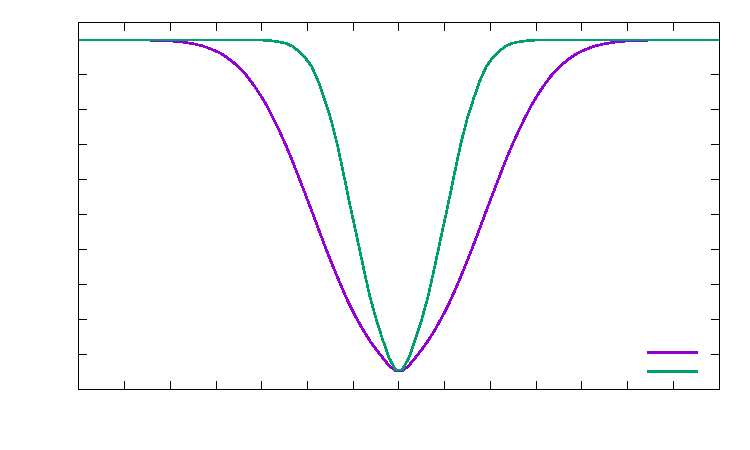
\includegraphics{questao1/powers}}%
    \gplfronttext
  \end{picture}%
\endgroup

  \caption{Poder do teste para diferentes médias reais}
  \label{fig:1-power}
\end{figure}

%%% Local Variables:
%%% mode: latex
%%% TeX-master: "../main"
%%% End:
